\section{Unterteilungen und Minoren}

\textbf{Definition}: Sei $G=(V,E)$ ein Graph, $e=uv$ eine Kante. Dann ist die \textbf{Unterteilung von $\boldsymbol{e}$ in $\boldsymbol{G}$} der Graph $G\circ e=(V',E')$ mit
\begin{itemize}
	\item $V'=V+\{w\}$
	\item $E'=(E\setminus \{uv\})+\{uw,vw\}$
\end{itemize}
\bigskip
\textbf{Beobachtung}: $G$ planar $\iff$ $G\circ e$ planar\\

\textbf{Definition}: Graph $G$ ist eine \textbf{Unterteilung von $\boldsymbol{H}$} wenn $G=((H \circ e_1)\circ e_2)\cdots)\circ e_k$.
Wir sagen auch $G$ ist $\boldsymbol{H}$\textbf{-Unterteilung}.
Graph $G$ \textbf{enthält eine $\boldsymbol{H}$-Unterteilung}, wenn ein Teilgraph $G'\subseteq G$ eine $H$-Unterteilung ist.

\begin{center}
	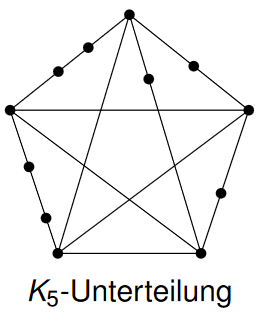
\includegraphics[width=0.17\textwidth]{images/k5-unterteilung.png}
\end{center}

\textbf{Beobachtung}: 
\begin{itemize}
	\item $K_5$- und $K_{3,3}$-Unterteilungen sind nicht-planar
	\item Jeder Graph der eine $K_5$ oder $K_{3,3}$-Unterteilung enthält, ist nicht planar
\end{itemize}
\bigskip
\textbf{Satz von Kuratowski}: $G$ ist planar $\iff$ $G$ enthält keine $K_5$- oder $K_{3,3}$-Unterteilung

\textit{Beweis}: \enquote{$\Rightarrow$} folgt aus obiger Beobachtung. Die Rückrichtung ist komplizierter und beweisen wir später.\\

\textbf{Definition}: Sei $G=(V,E)$ ein Graph, $e=uv$ eine Kante. Der Graph $G/e=(V',E')$ ist der Graph, der durch Kontrahieren der Kante $\boldsymbol{e}$ entsteht, genauer:
\begin{itemize}
	\item $V'=V\setminus\{u,v\}+\{w\}$
	\item $E'=E(G-u-v)\cup\{wa\mid au\in E \text{ oder } av\in E\}$
\end{itemize}
Diesen Prozess nennt man auch \textbf{Kantenkontraktion}. Dabei können Multikanten und Schlaufen entstehen.
\begin{center}
	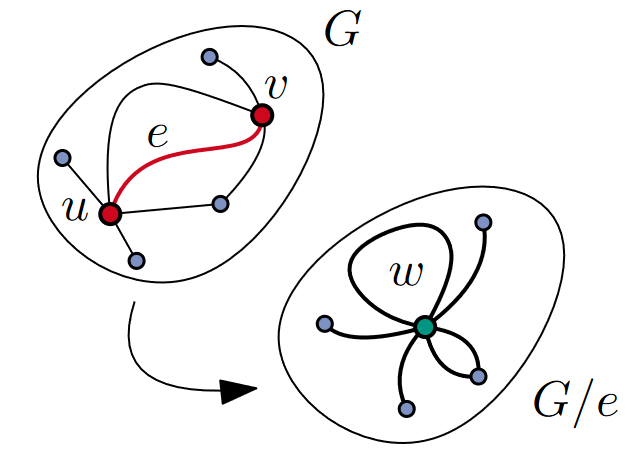
\includegraphics[width=0.3\textwidth]{images/kantenkontraktion.png}
\end{center}
\bigskip
\textbf{Definition}: Graph $H$ ist \textbf{Minor von} $\boldsymbol{G}$, wenn $H$ aus $G$ durch eine Folge von Kantenkontraktionen entsteht, also $H=((G/e_1)/e_2\cdots)/e_k$. Wir sagen dann auch: $G$ ist ein \textbf{$\boldsymbol{H}$-Minor} ($H$ ist der kleinere Graph, $G$ der Größere).\\

\textbf{Beobachtung}:
\begin{itemize}
	\item $G$ planar $\implies$ $G/e$ planar
	\item $G$ enthält $K_5$- oder $K_{3,3}$-Minor $\implies$ $G$ nicht planar
\end{itemize}
\bigskip
\textbf{Satz von Wagner}: $G$ planar $\iff$ $G$ enthält keinen $K_5$- oder $K_{3,3}$-Minor\\

\textbf{Lemma}: $G$ enthält $H$-Unterteilung $\implies $ $G$ enthält $H$-Minor

\textit{Beweis}: Kontrahiere durch Unterteilung entstandene Knoten zu ursprünglich adjazenten Knoten.
\begin{center}
	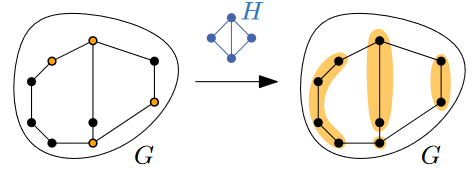
\includegraphics[width=0.35\textwidth]{images/um-skizze.png}
\end{center}
\pagebreak

\textbf{Es sind also äquivalent}:
\begin{enumerate}
	\item $G$ ist nicht planar
	\item $G$ enthält $K_5$- oder $K_{3,3}$-Minor
	\item $G$ enthält $K_5$- oder $K_{3,3}$-Unterteilung
\end{enumerate}

$(3)\implies(2)\implies(1)$ wurde schon bewiesen, $(1)\implies(2)\implies(3)$ müssen wir noch beweisen. Wir beginnen mit $(1)\implies(2)$.\\

\textit{Beweis von Wagner}: Es muss nur noch die Rückrichtung beweisen werden. Sei hierfür $G$ ein nicht-planarer Graph. Wir müssen einen $K_5$- oder $K_{3,3}$-Minor in $G$ finden. O.B.d.A. sei $G$ sogar minimal nicht-planar, d.h.
\begin{itemize}
	\item $G-v$ ist planar für jeden Knoten $v\in V$
	\item $G-e$ ist planar für jede Kante $e\in E$
	\item $G/e$ ist planar für jede Kante $e\in E$
\end{itemize}

Beweise zunächst folgendes Lemma:\\

\textbf{Lemma}: Sei $G$ minimal nicht-planar, $xy\in E(G)$. Dann ist $G-x-y$ ein Kreis.

\begin{wrapfigure}{r}{0.2\textwidth}
	\centering
	\vspace{30pt}
	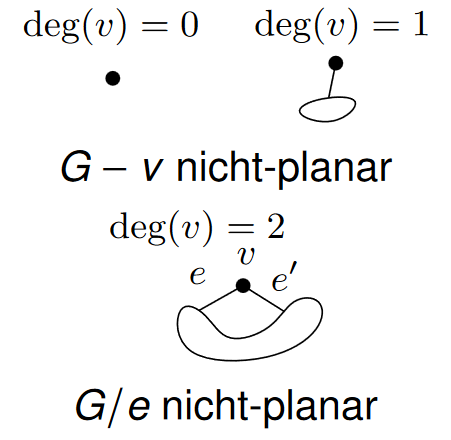
\includegraphics[width=0.22\textwidth]{images/wagner-1.png}
	\vspace{40pt}
	\vspace{-80pt}
\end{wrapfigure}
\textit{Beweis}: Da $G$ minimal nicht-planar ist,
\begin{itemize}
	\item ist $G$ zusammenhängend, da ansonsten Knoten aus einer Zusammenhangskomponente gelöscht werden könnte
	\item ist $\text{deg}(v)\geq 3$ für jeden Knoten $v\in V(G)$, denn Knoten von Grad 0 und 1 tragen nichts zur Nicht-Planarität bei, können also gelöscht werden ohne die Nicht-Planarität zu verlieren. Für einen Knoten $v$ von Grad 2 mit Kanten $e, e'$ bleibt $G/e$ nicht-planar. Wäre $G/e$ planar, so muss wegen $G = (G/e) \circ e'$ bereits $G$ planar sein. Widerspruch.
\end{itemize}

Das Lemma wird nun anhand von 3 Behauptungen bewiesen.\\

\underline{1. Behauptung}: $G-x-y$ enthält kein $\Theta$.

\textbf{Theta-Graphen} sind Unterteilungen des Graphen mit zwei Knoten und drei parallelen Kanten.
\begin{center}
	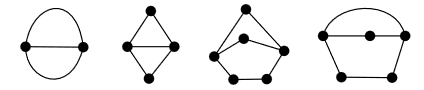
\includegraphics[width=0.3\textwidth]{images/theta.png}
\end{center}
\pagebreak


\textbf{Notation}: Für einen Kreis $C$ in einer planaren Zeichnung erhält man eine geschlossene \textbf{Jordankurve}, die die Ebene in zwei Komponenten unterteilt:
\begin{itemize}
	\item $\text{int}(C)$, das Innere von $C$
	\item $\text{ext}(C)$ , das Äußere von $C$
\end{itemize}
\begin{wrapfigure}{r}{0.25\textwidth}
	\centering
	\vspace{-70pt}
	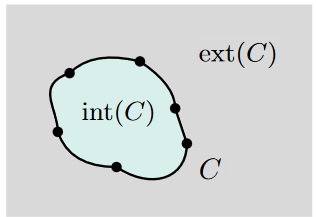
\includegraphics[width=0.22\textwidth]{images/jordan.png}
	\vspace{40pt}
	\vspace{-60pt}
\end{wrapfigure}

\textit{Beweis von Behauptung 1}:
\begin{itemize}
	\item Angenommen $G-x-y$ enthält ein $\Theta$.
	\item $G'\coloneqq G/xy$ ist planar mit Kante $xy$ zu Knoten $z$ kontrahiert.
	\item $G'-z=G-x-y$ ist ebenfalls planar.
	\item Zeichnung von $G'$ enthält ein $\Theta$ und das $\Theta$ hat 3 Kreise:
	\begin{center}
		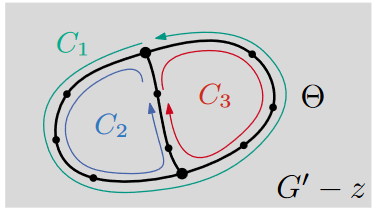
\includegraphics[width=0.3\textwidth]{images/wagner-2.png}
	\end{center}
	\item Betrachte Kreis $C$ im $\Theta$, sodass Knoten $z$ auf einer Seite von $C$ und eine Kante $e'\in E(\Theta)$ auf der anderen Seite von $C$ liegt.
	\item Wähle $\Theta$ und $C$ so, dass die Seite von $C$ mit $z$ inklusionsminimal ist, d.h. es gibt kein anderes $\Theta$ mit Kreis $C$, was $z$ enthält und ein kleineres Inneres hat
	\item O.B.d.A. gilt $z\in\text{int}(C)$ und $e'\in\text{ext}(C)$
	\begin{center}
		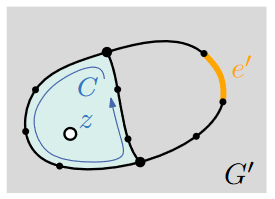
\includegraphics[width=0.27\textwidth]{images/wagner-3.png}
	\end{center}
	\item Betrachte $G''=G-\text{ext}(C)$.
	\item Da $e'\notin G''$ ist, wird mindestens eine Kante gelöscht, also ist $G''$ planar.
	\item Betrachte eine planare Zeichnung von $G''$ mit Kreis $C$.
\end{itemize}

\underline{Ziel}: Zeige, dass $C$ eine Facette berandet, denn dann kann $\text{ext}(C)$ in $C$ eingesetzt werden, was aber eine planare Zeichnung von $G$ wäre. \Lightning
\begin{center}
	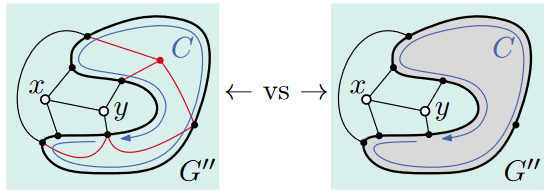
\includegraphics[width=0.4\textwidth]{images/wagner-4.png}
\end{center}

\begin{itemize}
	\item Betrachte Pfad $P$ in $G''$, der auf verschiedenen Knoten von $C$ startet und endet und ansonsten zu C disjunkt ist.
	\item $P$ entspricht auch einem Pfad $P'$ in $G'$.
\end{itemize}

Wenn $z\notin P'$:
\begin{itemize}
	\item Dann ist $C\cup P'$ ein $\Theta$ in $G-x-y$.
	\item Dieses $\Theta$ hat einen Kreis der $z$ enthält, aber ein kleineres Inneres als $C$ hat.
	\item Widerspruch zur Wahl von $\Theta$ und $C$.
\end{itemize}
\begin{center}
	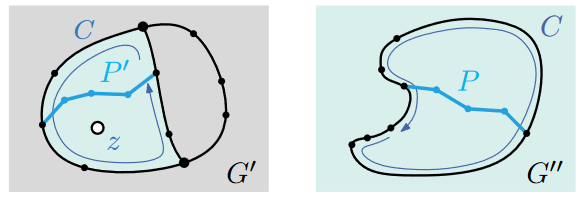
\includegraphics[width=0.4\textwidth]{images/wagner-5.png}
\end{center}

Also liegt $z$ auf $P'$ und $P$ muss $x$ oder $y$ enthalten. Also liegt jeder solche Pfad in der Zeichnung von $G''$ auf der Seite von $C$, die $xy$ enthält. 


$\implies$ $C$ liegt im Rand einer Facette von $G''$

Damit ist \textit{Behauptung 1} bewiesen.\\

\begin{wrapfigure}{r}{0.15\textwidth}
	\centering
	\vspace{-30pt}
	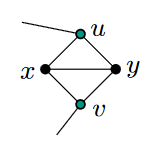
\includegraphics[width=0.15\textwidth]{images/wagner-7.png}
	\vspace{40pt}
	\vspace{-1000pt}
\end{wrapfigure}
\underline{2. Behauptung}: $G-x-y$ enthält keine zwei Knoten vom Grad 1.

\textit{Beweis von Behauptung 2}: 
\begin{itemize}
	\item Angenommen $u,v$ sind zwei Knoten in $G-x-y$ mit Grad 1.
	\item Da $\text{deg}(u),\text{deg}(v)\geq 3$ in $G$, sind $ux, uy, vx, vy \in E(G)$ und $u,v,x,y$ bilden ein $\Theta$
	\item Nach Behauptung 1 hat jede Kante in $G$ mindestens einen Endpunkt in $u, v, x, y$, um das $\Theta$ bei Kontraktion einer beliebigen Kante zu zerstören.
	\item Jedes $w\neq u, v, x, y$ ist zu $u$, $v$ oder beiden benachbart, da $\text{deg}(w)\geq 3$.
	\item Höchstens 2 Knoten außerhalb von $u, v, x, y$.
	\begin{center}
		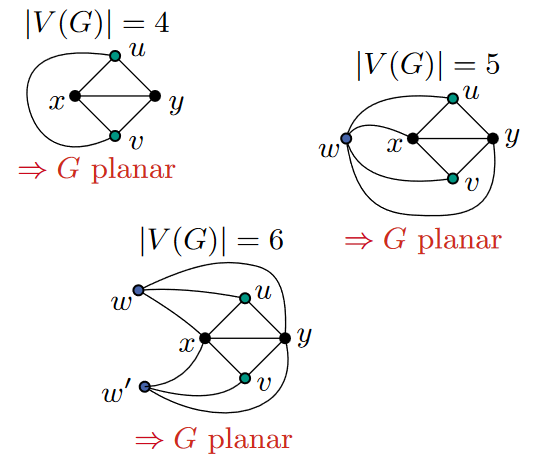
\includegraphics[width=0.4\textwidth]{images/wagner-8.png}
	\end{center}
\end{itemize}

$\implies$ In allen Fällen ergibt sich ein Widerspruch zur Nicht-Planarität von $G$.

Damit ist \textit{Behauptung 2} bewiesen.\\

\textbf{Definition}: Ein Graph enthält genau dann kein $\Theta$, wenn jede Kante auf höchstens einem Kreis liegt. Solche Graphen nennt man \textbf{Kakteen}. Kakteen sind kantendisjunkte Vereinigungen von Kreisen und Brücken.
\begin{center}
	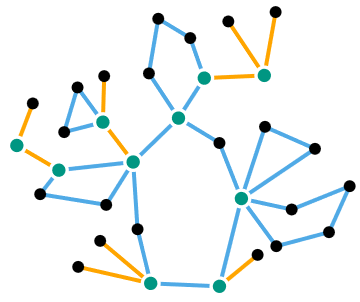
\includegraphics[width=0.25\textwidth]{images/kaktus.png}
\end{center}

\textbf{Definition}: Der \textbf{Block-Cutvertex-Tree} eines zusammenhängenden Graphen $G$ (hier ist $G$ Kaktus) ist ein Baum $T$ mit:
\begin{itemize}
	\item $V(T)=\{\text{\textcolor{teal}{Artikulationspunkt} in } G\}\cup\{\text{\textcolor{cyan}{Kreise} in } G\}\cup\{\text{\textcolor{orange}{Brücken} in } G\}$
	\item $E(T)=\{\textcolor{teal}{v}b\mid \textcolor{teal}{v}\text{ \textcolor{teal}{Artikulationspunkt}}, b \text{ \textcolor{orange}{Brücke}} \text{ oder } \text{\textcolor{cyan}{Kreis}}, \textcolor{teal}{v} \text{ Knoten auf } b \text{ in } G\}$
\end{itemize}
\begin{center}
	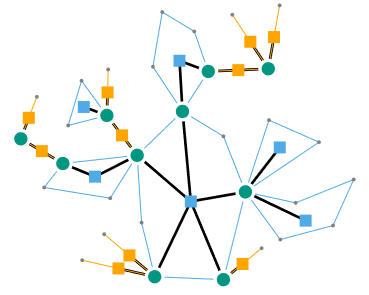
\includegraphics[width=0.28\textwidth]{images/bct.png}
\end{center}

\underline{Behauptung 3}: $G-x-y$ ist tatsächlich ein Kreis.

\textit{Beweis von Behauptung 3}:
\begin{itemize}
	\item Sei $T$ Block-Cutvertex-Tree von $G-x-y$.
	\item Wenn $G-x-y$ keinen Artikulationspunkt enthält, ist $G-x-y$ ein Kreis (Beweis fertig)  oder eine Kante. Dann gilt $|V(G)|\leq 4$, da $G$ höchstens nur die Knoten $x,y$ und die Endpunkte der Kante enthält
	$\implies$ $G$ ist planar \Lightning
	\item Also gibt es Artikulationspunkte und $|T|\geq 2$.
	\item Also hat $T$ mindestens 2 Blätter.
	\item Blätter im Block-Cutvertex-Tree sind entweder Brücken oder Kreise im ursprünglichen Graphen. Brücken führen immer zu Grad 1 Knoten. Nach Behauptung 2 gibt es ein Blatt in $T$, das in $G$ ein Kreis $C$ hat.
	\item Sei $v$ der Artikulationspunkt in $C$, der $C$ an den Graphen \enquote{klebt}.
	\item Jedes $u\in V(C)-v$ hat Grad 2 in $G-x-y$ (da Blatt im Cutvertex-Tree), aber mindestens Grad 3 in $G$.
	\item Also ist jedes $u$ zu $x$ oder $y$ benachbart. $u$ kann nicht zu beiden benachbart sein, da sonst $G-v-w$ ein $\Theta$ enthält.
	\begin{center}
		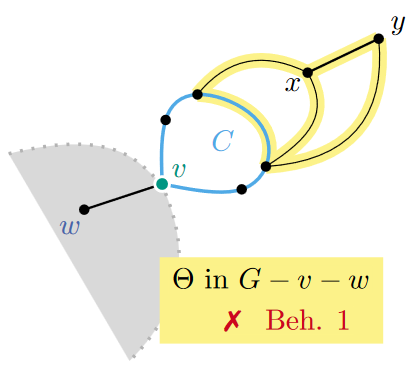
\includegraphics[width=0.27\textwidth]{images/wagner-9.png}
	\end{center}
	\item Ebenso darf $C$ nur Länge 3 haben, da sonst $G-v-w$ ebenso wieder ein $\Theta$ bildet.
	\begin{center}
		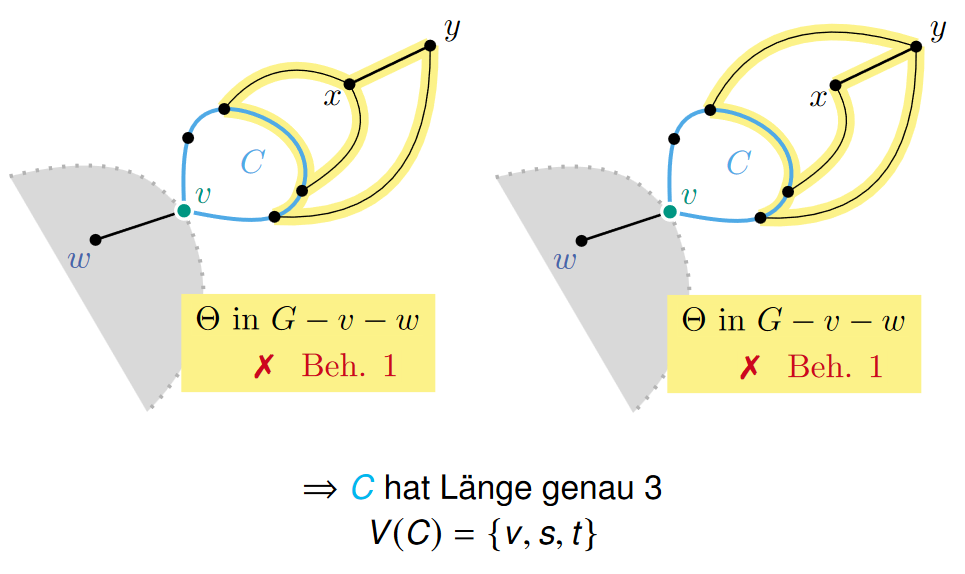
\includegraphics[width=0.5\textwidth]{images/wagner-10.png}
	\end{center}
	\item Dann hat $C\cup\{x,y\}$ ein $\Theta$ in $G$.
	\begin{center}
		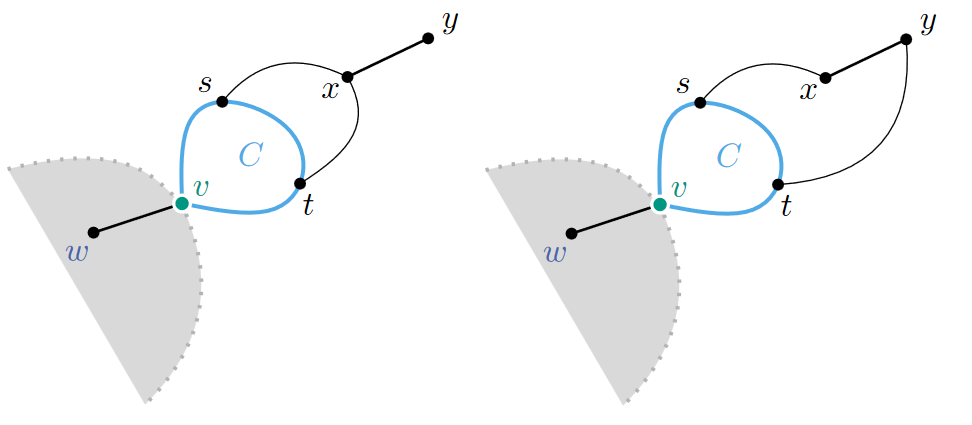
\includegraphics[width=0.5\textwidth]{images/wagner-11.png}
	\end{center}
	\item Nach Behauptung 1 hat jede Kante mindestens einen Endpunkt im $\Theta$. 
	\item Jedes $w\in G-(C\cup\{x,y\})$ hat alle Nachbarn in $C\cup\{x,y\}$, sonst gäbe es eine Kante außerhalb des $\Theta$. $w$ muss genau die Nachbarschaft $\{x,y,v\}$ haben, denn $w$ kann nicht zu $s$ oder $t$ benachbart sein, da diese Grad 2 haben.
	\item Würden zwei solche $w,w'$ existieren, so wäre $w,w',x,y$ ein $\Theta$ in $G-C$.
	\begin{center}
		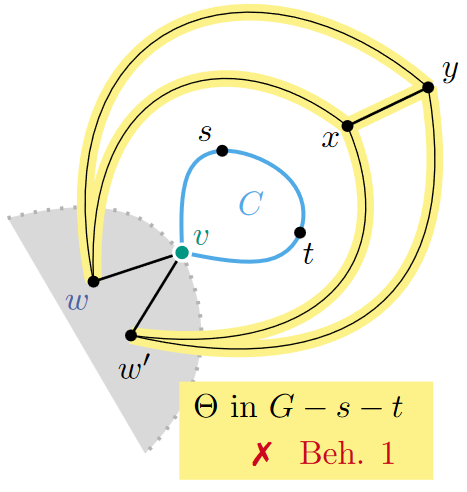
\includegraphics[width=0.27\textwidth]{images/wagner-12.png}
	\end{center}
	
	$\implies$ Also ist $w$ der einzige Knoten in $G-(C\cup\{x,y\})$.
	\item O.B.d.A sei $sx\in E$. Es gilt entweder $ty\in E$ oder $tx\in E$.
		\begin{center}
		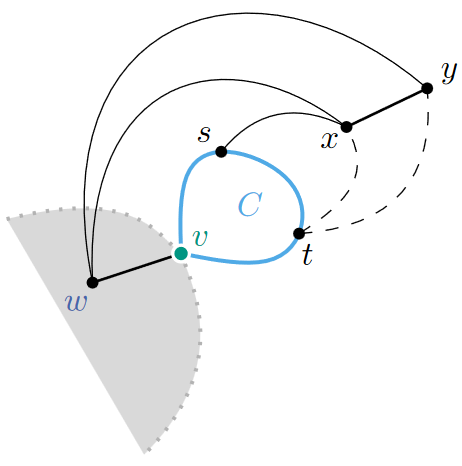
\includegraphics[width=0.27\textwidth]{images/wagner-13.png}
	\end{center}
	\item Wir wissen, dass $G$ nur die Knoten $v, s, t, x, y, w$ besitzt.
	\item Wenn $vx\in E$ der $vy\in E$, dann gibt es ein $\Theta$ in $G-s-t$.
	\begin{center}
		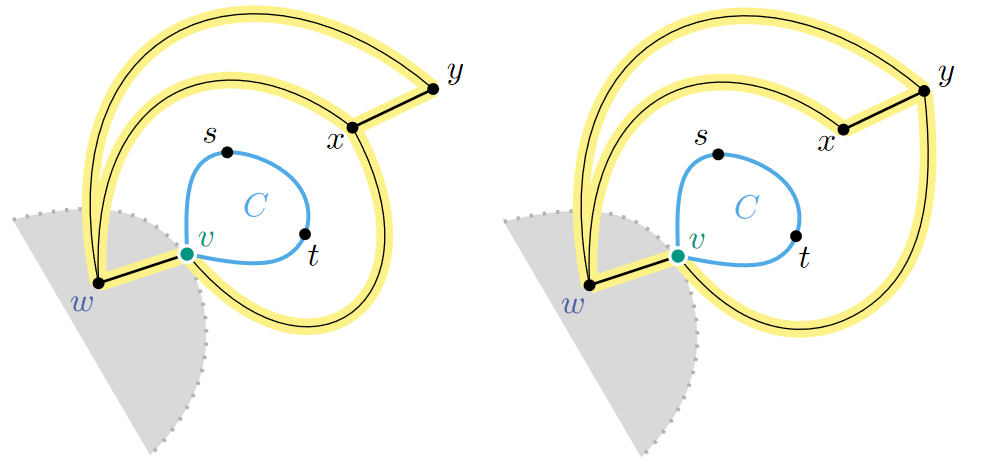
\includegraphics[width=0.5\textwidth]{images/wagner-14.png}
	\end{center}
	\item Wenn $tx\in E$, dann gibt es ein $\Theta$ in $G-w-y$.
	\begin{center}
		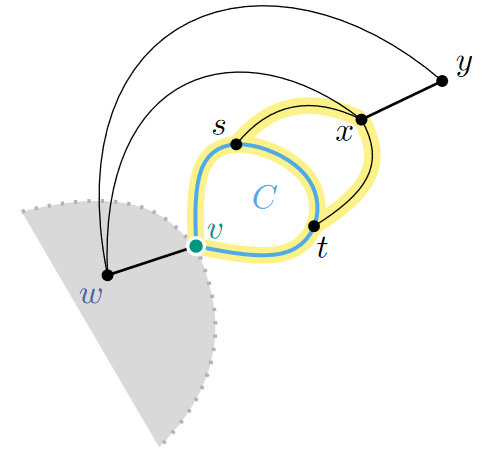
\includegraphics[width=0.27\textwidth]{images/wagner-15.png}
	\end{center}
	\pagebreak

	\item Insgesamt wissen wir $vx\notin E, vy\notin E, tx\notin E, ty\in E, ws\notin E, wt\notin E$. Wir kennen also ganz $G$ und $G$ ist planar. Widerspruch.
	\begin{center}
		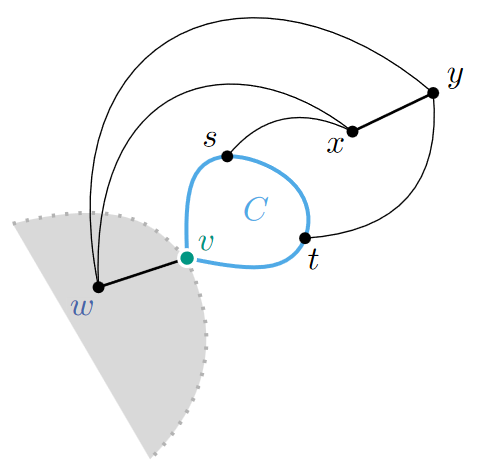
\includegraphics[width=0.27\textwidth]{images/wagner-16.png}
	\end{center}
\end{itemize}

Damit sind \textit{Behauptung 3} und das \textit{Lemma} bewiesen.\\

\textit{Beweis von Wagner - Abschluss}: 
\begin{itemize}
	\item Sei $xy\in E$ eine Kante und $C$ der Kreis $G-x-y$.
	\item Sei $uv\in E$ eine Kante auf $C$ mit $ux\in E$.
\end{itemize}

1. Fall: $uy\notin E$.
\begin{itemize}
	\item $G-u-x$ ist ein Kreis, d.h. $v$ muss Grad 2 haben, also ist $vy\in E$.
	\begin{center}
		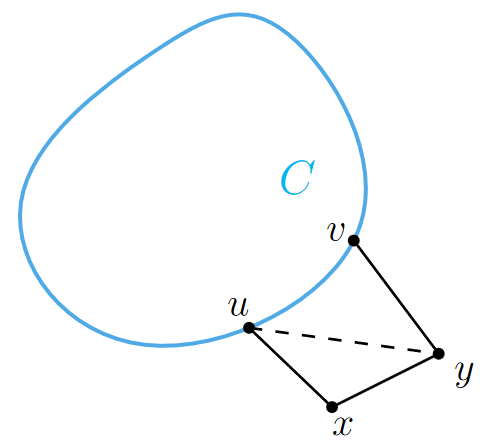
\includegraphics[width=0.25\textwidth]{images/wagner-17.png}
	\end{center}
	\item Wenn $vx\in E$ dann hat $G-x-v$ einen Knoten $u$ mit Grad 1. \Lightning
	
	$\implies vx\notin E$
	\item Analoge Argumente liefern: $N(x), N(y)$ sind auf $C$ disjunkt und alternierend.
	\item $|C|\geq 4$ und wir finden einen $K_{3,3}$-Minor.
	\begin{center}
		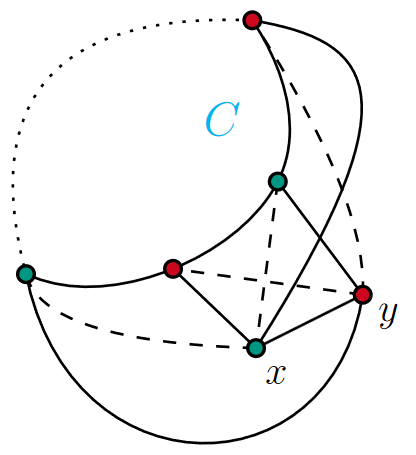
\includegraphics[width=0.23\textwidth]{images/wagner-18.png}
	\end{center}
\end{itemize}

2. Fall: Jeder Knoten auf $C$ ist zu $x$ und $y$ benachbart.
\begin{itemize}
	\item $|C|\geq 3$. Wir finden einen $K_5$-Minor.
	\begin{center}
		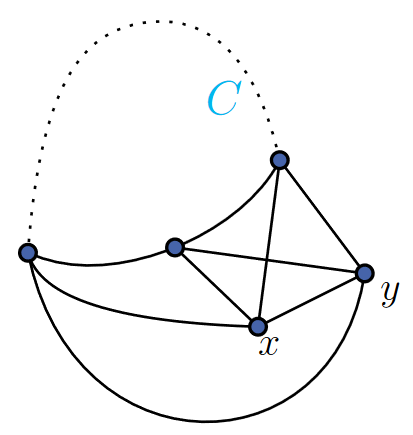
\includegraphics[width=0.23\textwidth]{images/wagner-19.png}
	\end{center}
\end{itemize}

Damit ist der \textbf{Satz von Wagner} bewiesen.\\

Wir beweisen nun (2) $\implies$ (3).\\

\textbf{Lemma}: Seien $G,H$ Graphen. Maximaler Grad von $H$ höchstens 3, d.h. $\Delta(H)\leq 3$. Dann sind äquivalent:
\begin{itemize}
	\item $G$ enthält $H$-Minor
	\item $G$ enthält $H$-Unterteilung
\end{itemize}

\textit{Beweis}: Die Richtung Unterteilung $\implies$ Minor wurde bereits gezeigt. Beweise nun also die Rückrichtung. In einem $H$-Minor finden wir $H$-Unterteilung.
\begin{itemize}
	\item O.B.d.A ist ist jede Kontraktionsmenge ein Baum, sodass
	\begin{itemize}
		\item jedes Blatt hat Nachbarn in anderer Menge,
		\item zwischen je zwei Mengen ist maximal eine Kante
	\end{itemize}
	Überflüssige Kanten können gelöscht werden.
	\item Wähle Knoten von maximalem Grad in jeder Menge.
	\item Dann bilden diese Bäume schon eine H-Unterteilung, da $\Delta(H)\leq 3$.
	\begin{center}
		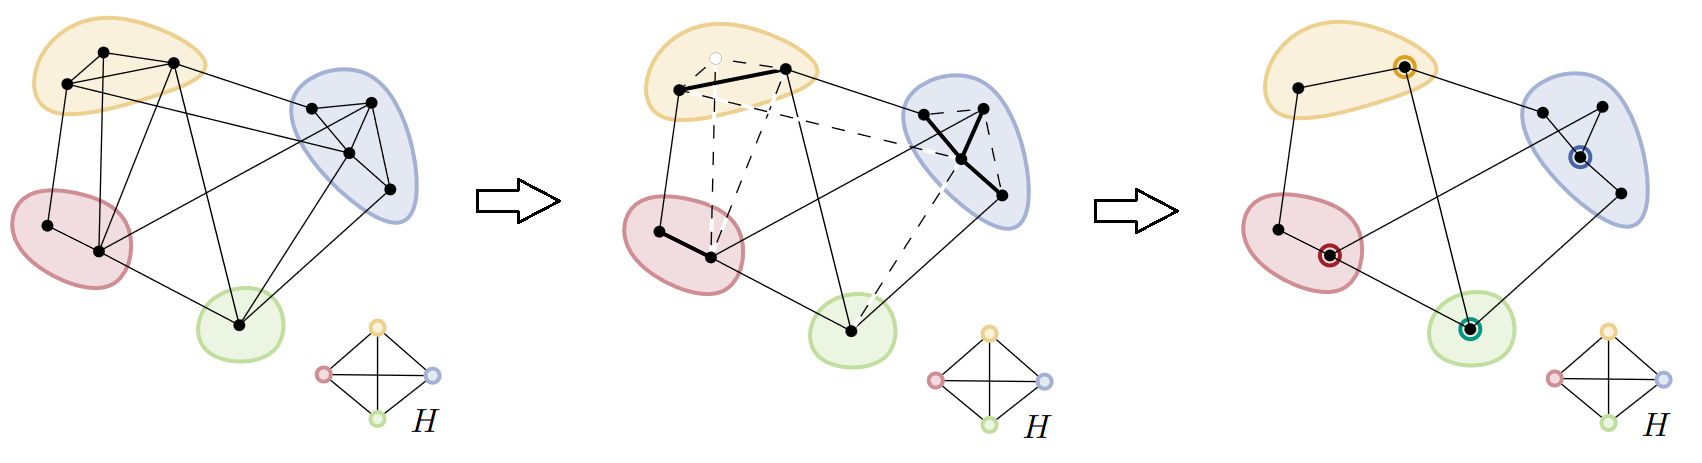
\includegraphics[width=0.8\textwidth]{images/m-u.png}
	\end{center}
\end{itemize}
\pagebreak

\textit{Beweis von Kuratowski}: Es muss nur noch die Richtung $G$ nicht planar $\implies$ $G$ enthält eine $K_5$ oder $K_{3,3}$-Unterteilung bewiesen werden.
\begin{itemize}
	\item Sei also $G$ nicht planar. Wir müssen Unterteilung von $K_{3,3}$ oder $K_5$ finden.
	\item Nach Wagner gibt es einen $K_{3,3}$- oder $K_5$-Minor in $G$.
	\item Bei $K_{3,3}$-Minor, sind wir nach vorigem Lemma fertig.
\end{itemize}
Sonst: Induktion über Knotenzahl von $G$:
\begin{itemize}
	\item I.A.: $G$ muss mindestens $5$ Knoten besitzen, um nicht-planar zu sein, und dort kommt auch nur $K_5$ in Frage.
	\item I.S.: Wenn es sich beim $K_5$-Minor um einen $K_5$-Teilgraph handelt, dann sind wir fertig. Andernfalls gibt es $e = uv$, sodass $G / e$ immer noch einen $K_5$-Minor enthält. $G/e$ ist also immer noch nicht-planar. Nach IV existiert eine $K_{3,3}$- oder $K_5$-Unterteilung in $G/ e$. Sei $w$ der Knoten, zu dem $e$ kontrahiert wird. 
	\begin{itemize}
		\item Wenn $w$ in der Unterteilung ein Unterteilungspunkt ist (also $\text{deg}(w)=2$), gibt es auch solch eine Unterteilung in $G$.
		\item Wenn $\text{deg}(w)=3$ in Unterteilung, gibt es auch in $G$ eine Unterteilung.
		\begin{center}
			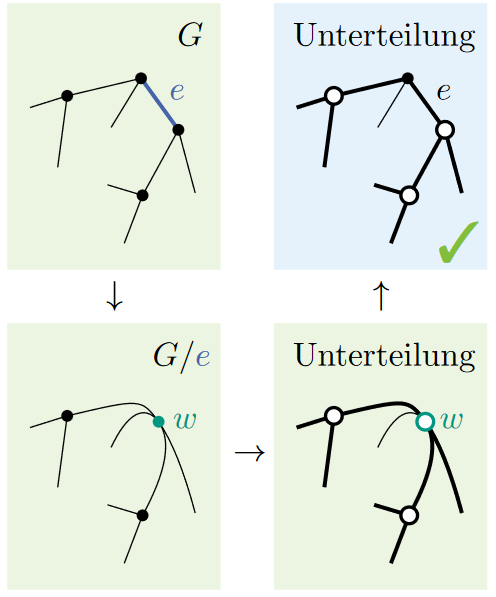
\includegraphics[width=0.29\textwidth]{images/kuratowski-1.png}
		\end{center}
	\item Also o.B.d.A. $\text{deg}(w)=4$ in $K_5$-Unterteilung in $G/e$.
	\begin{center}
		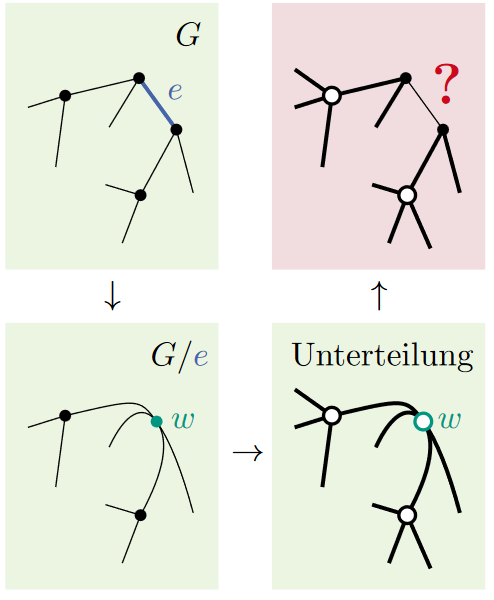
\includegraphics[width=0.3\textwidth]{images/kuratowski-2.png}
	\end{center}
	\item Betrachte die vier anderen Knoten von Grad 4.
	\item Sind mindestens drei davon zu $u$ verbunden, finden wir wieder eine $K_5$-Unterteilung in $G$.
	\begin{center}
		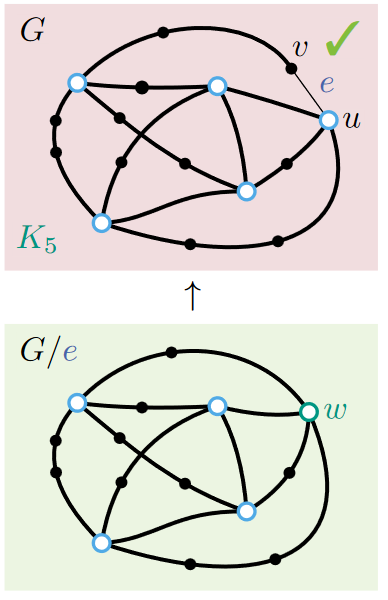
\includegraphics[width=0.2\textwidth]{images/kuratowski-3.png}
	\end{center}
	\item Andernfalls sind zwei zu $u$ und zwei zu $v$ verbunden und wir finden eine $K_{3,3}$-Unterteilung in $G$.
	\begin{center}
		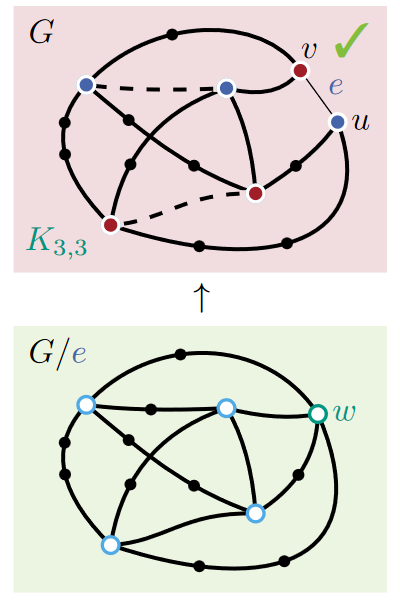
\includegraphics[width=0.2\textwidth]{images/kuratowski-4.png}
	\end{center}
	\end{itemize}
\end{itemize}

Damit wurde der \textbf{Satz von Kuratowski} bewiesen.